\documentclass[11pt]{article}

\usepackage[a4paper,margin=3cm]{geometry} % For page dimensions
\usepackage{fontspec} % For font selection
\usepackage{unicode-math} % For mathematical fonts
\usepackage{polyglossia} % For language selection
\usepackage{graphicx} % For images
\usepackage[colorlinks=true, linkcolor=black, urlcolor=blue, citecolor=green]{hyperref} % For hyperlinks
\usepackage{xcolor} % Colors for code highlighting
\usepackage{fancyhdr} % For headers and footers
\usepackage{bookmark}
\usepackage{nameref} % For referencing sections
\usepackage{draftwatermark} % For watermarks
\usepackage{amsmath} % For mathematical equations
\usepackage{listings} % For code formattings
\usepackage{tikz} % For diagrams
\usepackage{subcaption} % For subfigures
\usepackage{float} % For floating figures

\graphicspath{ {images} }

% Set fonts
% \setmainfont{Noto Serif}
\setromanfont{Noto Serif}
\setsansfont{Noto Sans}
\setmonofont{Noto Sans Mono}

% Set languages
\setmainlanguage{greek}
\setotherlanguages{english}

% Header and footer settings
\pagestyle{fancy}
\setlength{\headheight}{14pt}
\fancyhf{}
\fancyfoot[C]{\thepage}

% Custom Commands
\newcommand{\email}[1]{\href{mailto://#1}{\texttt{#1}}} % Email formatting
\newcommand{\developer}[2]{#1 (#2) \\ \email{up#2@ac.upatras.gr} \\[2ex]}
\newcommand{\appname}{Loop}

\author{
    \developer{Γιάννης Ραβασόπουλος}{1100696}
    \developer{Κώστας Λουκανάρης}{1100610}
    \developer{Χρήστος Μάριος Νικολόπουλος}{1100644}
    \developer{Άγγελος Αβεντισιάν}{1100491}
    \developer{Βασίλης Μυλωνάς}{1100643}
}

\date{
    \today \\[1ex]
    Έκδοση 0.1 \\
}

% For pandoc
\providecommand{\tightlist}{%
    \setlength{\itemsep}{0pt}\setlength{\parskip}{0pt}}


\fancyhead[L]{Περιγραφή Έργου}
\fancyhead[R]{\leftmark}

\title{
     Εφαρμογή \appname\\[1ex]
    \large Τεχνολογία Λογισμικού - ΤΜΗΥΠ, Πανεπιστήμιο Πατρών \\[2ex]
}

\begin{document}

\maketitle
\thispagestyle{empty}
\newpage

\tableofcontents
\newpage

\begin{abstract}
    Περιγραφή ανάπτυξης συστήματος και συνοδεύουσας εφαρμογής για την διευκόλυνση
    συνεπιβίβασης σε κοινές διαδρομές (carpooling). Η εφαρμογή εγκαθισταται σε
    κινητές συσκευές και παρέχει ζωντανή πληροφόρηση
    αντλώντας πληροφορίες από τους χρήστες. H εφαρμογή απευθύνεται αμφότερα σε
    οδηγούς αυτοκινήτων αλλά και σε πεζούς. Στόχος είναι η καλύτερη αξιοποίηση
    του οδικού δικτύου και η μείωση της κυκλοφοριακής συμφόρησης σε αστικές
    περιοχές.
\end{abstract}

\newpage

\section{Περιγραφή}

\subsection{Περιγραφή του Προβλήματος}

Είναι γνωστό ότι το μεγαλύτερο μέρος του αστικού πληθυσμού είναι άτομα τα
οποία έχουν καθημερινές υποχρεώσεις και πρέπει να βρίσκονται
σε συγκεκριμένα μέρη σε συγκεκριμένες ώρες. Χαρακτηριστικό παράδειγμα είναι οι
φοιτητές και οι εργαζόμενοι οι οποίοι έχουν συνήθως προκαθορισμένο ωράριο και
πρόγραμμα.

Πολλοί από αυτούς επιλέγουν την αυτοκίνηση λόγω της κακής κατάστασης των μέσων
μαζικής μεταφοράς. Ενδεικτικά είναι τα λεωφορεία με δρομολόγια
προς το πανεπιστήμιο τα οποία είναι γεμάτα τις πρωινές ώρες. Η αύξηση όμως της
χρήσης των αυτοκινήτων οδηγεί σε αύξηση της κυκλοφοριακής συμφόρησης και
της ατμοσφαιρικής ρύπανσης.

\subsection{Προτεινόμενη Λύση}

Η προτεινόμενη λύση είναι η ανάπτυξη μίας εφαρμογής για κινητές συσκευές
η οποία θα διευκολύνει τους χρήστες να μοιράζονται οχήματα (carpooling) στις
διαδρομές τους. Μοιράζοντας οχήματα σε κοινές διαδρομές η χρήστες μειώνουν
την κυκλοφοριακή συμφόρηση και ταυτόχρονα το κόστος μεταφοράς τους.

Σαν επιπλέον όφελος προτείνεται η υλοποίηση ενός συστήματος πόντων και ανταμοιβών
υπό την μορφή κουπονιών το οποίο θα ενθαρρύνει τους χρήστες να συμμετάσχουν
στην εφαρμογή.

\newpage

\section{Σύσταση Ομάδας}
Η ομάδα αποτελείται από 5 μέλη, με ρόλους που καθορίστηκαν βάσει της εμπειρίας και των ενδιαφερόντων:
\begin{itemize}
    \item Βασίλης Μυλωνάς (Επικεφαλής Έργου / Project Manager)
    \item Άγγελος Αβεντισιάν (Υπεύθυνος Ποιότητας / QA Manager)
    \item Γιάννης Ραβασόπουλος
    \item Κώστας Λουκανάρης
    \item Χρήστος Μάριος Νικολόπουλος
\end{itemize}

\newpage

\section{Απαιτήσεις}

\subsection{Λειτουργικές Απαιτήσεις}

\begin{enumerate}
    \item Ο χρήστης πρέπει να μπορεί να εγγραφεί και να συνδεθεί μέσω πολλαπλών μεθόδων (email, Google, Facebook).
    \item Ο χρήστης πρέπει να μπορεί να δηλώνει δραστηριότητες, παρέχοντας πληροφορίες όπως τοποθεσία και ώρες.
    \item Να υπάρχει η δυνατότητα αναζήτησης άλλων χρηστών με όμοιες διαδρομές.
    \item Να δίνεται η δυνατότητα επικοινωνίας μεταξύ των χρηστών για τον καθορισμό σημείου συνάντησης.
    \item Να εφαρμόζεται σύστημα βαθμολόγησης και σχολιασμού, τόσο για οδηγούς όσο και για επιβάτες.
    \item Η εφαρμογή θα πρέπει να παρέχει ανταμοιβές υπό τη μορφή κουπονιών ως κίνητρο χρήσης.
\end{enumerate}

\subsection{Μη Λειτουργικές Απαιτήσεις}

\begin{enumerate}
    \item Η αναζήτηση και οι ενημερώσεις δεδομένων θα πρέπει να γίνονται σε πραγματικό χρόνο.
    \item Πρέπει να διασφαλίζεται η ασφάλεια των επιβατών και των οδηγών μέσω ελέγχου ταυτότητας
          και επαλήθευσης χρηστών.
    \item Το σύστημα πρέπει να υποστηρίζει μελλοντικές επεκτάσεις με πρόσθεση νέων λειτουργιών.
    \item Η διεπαφή θα πρέπει να είναι φιλική και εύχρηστη για όλους τους χρήστες.
\end{enumerate}

\newpage

% \input{generated}
\section{Use Case Descriptions}
\input{build/use-case/arrange-pickup.tex}
\input{build/use-case/confirm-pickup.tex}

\subsection{Create Activity}

Ο χρήστης επιθυμεί να δημιουργήσει μια δραστηριότητα στην εφαρμογή.

\subsubsection{Βασική Ροή}

\begin{enumerate}
    \item Ο χρήστης επιλέγει "Create Activity"
    \item Η εφαρμογή δημιουργεί μια κενή δραστηριότητα και την αποθηκεύει
          προσωρινά.
    \item Συνέχεια από το βήμα 2 της βασικής ροής του use case "Edit Activity".
\end{enumerate}

\input{build/use-case/create-ride.tex}
\subsubsection{Edit Activity}

\begin{enumerate}
    \item Ο χρήστης επιλέγει "Edit Activity".
    \item Η εφαρμογή εμφανίζει μενού με επιλογές για την ιδιότητα του χρήστη (πχ φοιτητής).
    \item Ο χρήστης επιλέγει την ιδιότητα του.
    \item Η εφαρμογή εμφανίζει την φόρμα αναζήτησης και έναν χάρτη της περιοχής του χρήστη.
    \item Ο χρήστης δηλώνει την περιοχή στην οποία επιθυμεί να μετακινηθεί.
    \item Η εφαρμογή εμφανίζει μενού με επιλογές για τις μέρες και τις ώρες έναρξης και λήξης
          της δραστηριότητας.
    \item Ο χρήστης εισάγει τα κατάλληλα στοιχεία.
    \item H εφαρμογή εμφανίζει μενού με επιλόγες για το μέσο μεταφοράς του χρήστη
    \item Ο χρήστης επιλέγει το μέσο μεταφοράς του.
    \item Το σύστημα εκτελεί προεπεξεργασία στα δεδομένα.
    \item Το σύστημα εισάγει την δραστηριότητα στο κατάλογο δραστηριοτήτων του χρήστη.
\end{enumerate}

\subsubsection{Εναλλακτική Ροή: Ακύρωση 1}

\begin{enumerate}
    \item[3] Ο χρήστης ακυρώνει την διαδικασία και επιστρέφει στην αρχική οθόνη.
\end{enumerate}

\subsubsection{Εναλλακτική Ροή: Ακύρωση 2}

\begin{enumerate}
    \item[5] Ο χρήστης ακυρώνει την διαδικασία και επιστρέφει στην αρχική οθόνη.
\end{enumerate}

\subsubsection{Εναλλακτική Ροή: Ακύρωση 3}

\begin{enumerate}
    \item[7] Ο χρήστης ακυρώνει την διαδικασία και επιστρέφει στην αρχική οθόνη.
\end{enumerate}

\subsubsection{Εναλλακτική Ροή: Ακύρωση 4}

\begin{enumerate}
    \item[9] Ο χρήστης ακυρώνει την διαδικασία και επιστρέφει στην αρχική οθόνη.
\end{enumerate}

\subsubsection{Εναλλακτική Ροή: Μη έγκυρα στοιχεία}

\begin{enumerate}
    \item[7] Ο χρήστης εισάγει μη έγκυρα στοιχεία.
    \item[8] Το σύστημα εμφανίζει μήνυμα σφάλματος και ζητά διόρθωση.
    \item[9] Συνέχεια από το βήμα 6 της βασικής ροής.
\end{enumerate}

\hypertarget{edit-profile}{%
\subsection{Edit Profile}\label{edit-profile}}

\hypertarget{ux3c0ux3b5ux3c1ux3b9ux3b3ux3c1ux3b1ux3c6ux3ae}{%
\subsubsection{Περιγραφή}\label{ux3c0ux3b5ux3c1ux3b9ux3b3ux3c1ux3b1ux3c6ux3ae}}

Ο χρήστης επιθυμεί να ενημερώσει τα στοιχεία του προφίλ του.

\hypertarget{ux3b2ux3b1ux3c3ux3b9ux3baux3ae-ux3c1ux3bfux3ae}{%
\paragraph{Βασική
Ροή}\label{ux3b2ux3b1ux3c3ux3b9ux3baux3ae-ux3c1ux3bfux3ae}}

\begin{enumerate}
\def\labelenumi{\arabic{enumi}.}
\tightlist
\item
  Ο χρήστης επιλέγει ``Profile'' στην οθόνη Account.
\item
  Το σύστημα ανακτά τα στοιχεία προφίλ του χρήστη και τα εμφανίζει στην
  οθόνη Profile.
\item
  Ο χρήστης τροποποιεί κάποια στοιχεία στην οθόνη Profile.
\item
  Το σύστημα εμφανίζει τον διάλογο επιβεβαίωσης τροποποίησης.
\item
  Ο χρήστης επιλέγει ``Confirm'' στον διάλογο επιβεβαίωσης τροποποίησης.
\item
  Το σύστημα ελέγχει την απάντηση του χρήστη.
\item
  Το σύστημα επαληθεύει τα στοιχεία.
\item
  To σύστημα ενημερώνει τα στοιχεία προφίλ του χρήστη.
\item
  Το σύστημα εμφανίζει μήνυμα επιτυχίας στην οθόνη Account.
\end{enumerate}

\hypertarget{ux3b5ux3bdux3b1ux3bbux3bbux3b1ux3baux3c4ux3b9ux3baux3ae-ux3c1ux3bfux3ae-ux3b1ux3baux3cdux3c1ux3c9ux3c3ux3b7}{%
\paragraph{Εναλλακτική Ροή:
Ακύρωση}\label{ux3b5ux3bdux3b1ux3bbux3bbux3b1ux3baux3c4ux3b9ux3baux3ae-ux3c1ux3bfux3ae-ux3b1ux3baux3cdux3c1ux3c9ux3c3ux3b7}}

\begin{enumerate}
\def\labelenumi{\arabic{enumi}.}
\setcounter{enumi}{4}
\tightlist
\item
  Ο χρήστης επιλέγει ``Cancel'' στον διάλογο επιβεβαίωσης τροποποίησης.
\item
  Το σύστημα ελέγχει την απάντηση του χρήστη.
\item
  Τo σύστημα επιστρέφει στην οθόνη Account.
\end{enumerate}

\hypertarget{ux3b5ux3bdux3b1ux3bbux3bbux3b1ux3baux3c4ux3b9ux3baux3ae-ux3c1ux3bfux3ae-ux3b1ux3c0ux3bfux3c4ux3c5ux3c7ux3afux3b1-ux3b5ux3c0ux3b1ux3bbux3aeux3b8ux3b5ux3c5ux3c3ux3b7ux3c2}{%
\paragraph{Εναλλακτική Ροή: Αποτυχία
Επαλήθευσης}\label{ux3b5ux3bdux3b1ux3bbux3bbux3b1ux3baux3c4ux3b9ux3baux3ae-ux3c1ux3bfux3ae-ux3b1ux3c0ux3bfux3c4ux3c5ux3c7ux3afux3b1-ux3b5ux3c0ux3b1ux3bbux3aeux3b8ux3b5ux3c5ux3c3ux3b7ux3c2}}

\begin{enumerate}
\def\labelenumi{\arabic{enumi}.}
\setcounter{enumi}{6}
\tightlist
\item
  Το σύστημα αποτυγχάνει να επαληθεύσει τα στοιχεία.
\item
  Το σύστημα εμφανίζει μήνυμα αποτυχίας στην οθόνη Profile.
\end{enumerate}

\hypertarget{ux3b1ux3bdux3acux3bbux3c5ux3c3ux3b7-ux3b5ux3c5ux3c1ux3c9ux3c3ux3c4ux3afux3b1ux3c2}{%
\subsubsection{Ανάλυση
Ευρωστίας}\label{ux3b1ux3bdux3acux3bbux3c5ux3c3ux3b7-ux3b5ux3c5ux3c1ux3c9ux3c3ux3c4ux3afux3b1ux3c2}}

\begin{figure}
\centering
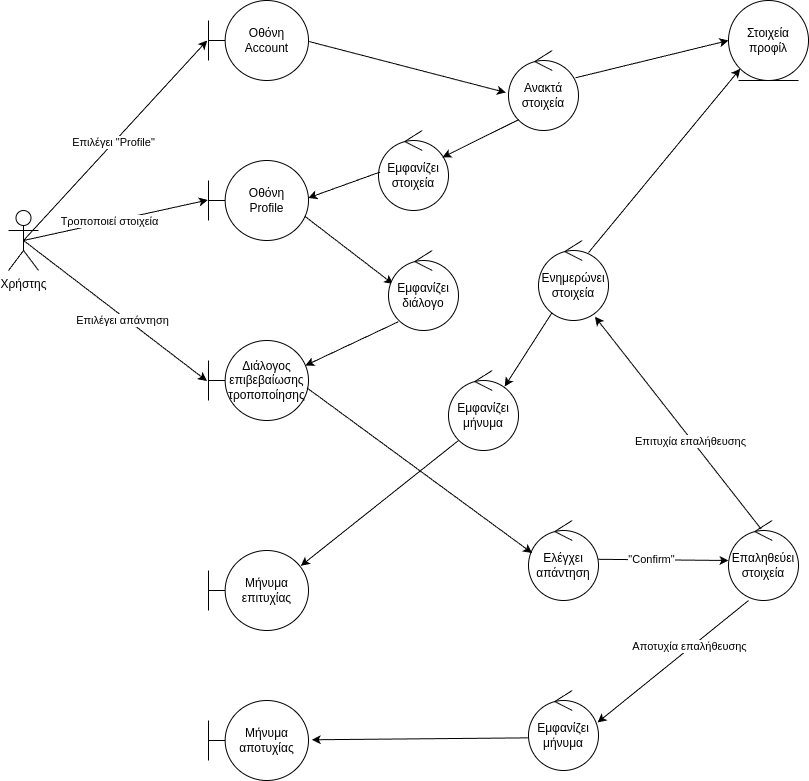
\includegraphics{./edit-profile-robustness.drawio.png}
\caption{image}
\end{figure}

\subsection{Find Ride}

Ο χρήστης επιθυμεί να βρεί οδηγό με κοινή διαδρομή με αυτόν για να συμμετέχει σε
κάποια δραστηριότητα (εργασία, μάθημα κλπ).

\subsubsection{Βασική Ροή}
\begin{enumerate}
    \item Ο χρήστης επιλέγει "Find Ride"
    \item Η εφαρμογή εμφανίζει τις δραστηριότητες του χρήστη.
    \item Ο χρήστης επιλέγει μια δραστηριότητα.
    \item To σύστημα εκτελεί αναζήτηση με βάση τα κριτήρια του χρήστη για δραστηριότητες
          άλλων χρηστών που εμφανίζουν τοπική και χρονική ομοιότητα.
    \item Το σύστημα κατατάσει τις δραστηριότητες με βάση την ομοιότητα.
    \item Το σύστημα εμφανίζει τις δραστηριότητες που βρέθηκαν.
    \item Ο χρήστης επιλέγει μια δραστηριότητα.
    \item Το σύστημα εμφανίζει τα στοιχεία του χρήστη που έχει δηλώσει την δραστηριότητα.
    \item Ο χρήστης επιλέγει "Pool".
    \item Το σύστημα ειδοποιεί τον δέκτη και ο χρήστης περιμένει την επιβεβαίωση του.
    \item O δέκτης αποδέχεται την πρόταση του χρήστη.
    \item Το σύστημα ενημερώνει τον χρήστη για τον επιτυχή προγραμματισμό.
\end{enumerate}

\subsubsection{Εναλλακτική Ροή: Ακύρωση 1}

\begin{enumerate}
    \item[3] Ο χρήστης ακυρώνει την αναζήτηση και επιστρέφει στην αρχική οθόνη.
\end{enumerate}

\subsubsection{Εναλλακτική Ροή: Ακύρωση 2}

\begin{enumerate}
    \item[7] Ο χρήστης ακυρώνει την αναζήτηση και επιστρέφει στην αρχική οθόνη.
\end{enumerate}

\subsubsection{Εναλλακτική Ροή: Ακύρωση 3}

\begin{enumerate}
    \item[9] Ο χρήστης αλλάζει γνώμη και πατάει "επιστροφή".
    \item[10] Συνέχεια από το βήμα 6 της βασικής ροής.
\end{enumerate}

\subsubsection{Εναλλακτική Ροή: Απόρριψη Πρότασης}

\begin{enumerate}
    \item[11] Ο δέκτης απορρίπτει την πρόταση του χρήστη.
    \item[12] Συνέχεια από το βήμα 6 της βασικής ροής.
\end{enumerate}

\subsubsection{Εναλλακτική Ροή: Εσωτερικό Σφάλμα}

\begin{enumerate}
    \item[5] Προκύπτει εσωτερικό σφάλμα κατά την αναζήτηση.
    \item[6] Το σύστημα ενημερώνει τον χρήστη για το σφάλμα και προτρέπει τον
        χρήστη σε αναφορά σφάλματος.
\end{enumerate}

\subsubsection{Εναλλακτική Ροή: Ο χρήστης δεν έχει δραστηριότητες}

\begin{enumerate}
    \item[2] Η εφαρμογή προτείνει την δημιουργία μιας δραστηριότητας.
    \item[3] Συνέχεια από το βήμα 1 της βασικής ροής του "Create Activity".
\end{enumerate}

\subsubsection{Εναλλακτική Ροή: Δεν βρέθηκαν όμοιες δραστηριότητες}

\begin{enumerate}
    \item[5] Το σύστημα δεν βρίσκει καμία δραστηριότητα που να ταιριάζει με τα
        κριτήρια του χρήστη.
    \item[6] Το σύστημα ενημερώνει τον χρήστη για την αποτυχία και προτείνει
        τροποποίηση της δραστηριότητας ή τη χρήση δημόσιας συγκοινωνίας.
    \item[7] Ο χρήστης επιλέγει "ΟΚ" και επιστρέφει στην αρχική οθόνη.
\end{enumerate}


\subsection{Create Activity}

Ο χρήστης επιθυμεί να δημιουργήσει μια δραστηριότητα στην εφαρμογή.

\subsubsection{Βασική Ροή}

\begin{enumerate}
    \item Ο χρήστης επιλέγει "Create Activity"
    \item Η εφαρμογή δημιουργεί μια κενή δραστηριότητα και την αποθηκεύει
          προσωρινά.
    \item Συνέχεια από το βήμα 2 της βασικής ροής του use case "Edit Activity".
\end{enumerate}


\subsubsection{Edit Activity}

\begin{enumerate}
    \item Ο χρήστης επιλέγει "Edit Activity".
    \item Η εφαρμογή εμφανίζει μενού με επιλογές για την ιδιότητα του χρήστη (πχ φοιτητής).
    \item Ο χρήστης επιλέγει την ιδιότητα του.
    \item Η εφαρμογή εμφανίζει την φόρμα αναζήτησης και έναν χάρτη της περιοχής του χρήστη.
    \item Ο χρήστης δηλώνει την περιοχή στην οποία επιθυμεί να μετακινηθεί.
    \item Η εφαρμογή εμφανίζει μενού με επιλογές για τις μέρες και τις ώρες έναρξης και λήξης
          της δραστηριότητας.
    \item Ο χρήστης εισάγει τα κατάλληλα στοιχεία.
    \item H εφαρμογή εμφανίζει μενού με επιλόγες για το μέσο μεταφοράς του χρήστη
    \item Ο χρήστης επιλέγει το μέσο μεταφοράς του.
    \item Το σύστημα εκτελεί προεπεξεργασία στα δεδομένα.
    \item Το σύστημα εισάγει την δραστηριότητα στο κατάλογο δραστηριοτήτων του χρήστη.
    \item Η εφαρμογή εμφανίζει μήνυμα επιτυχίας.
\end{enumerate}

\subsubsection{Εναλλακτική Ροή: Ακύρωση 1}

\begin{enumerate}
    \item[3] Ο χρήστης ακυρώνει την διαδικασία και επιστρέφει στην αρχική οθόνη.
\end{enumerate}

\subsubsection{Εναλλακτική Ροή: Ακύρωση 2}

\begin{enumerate}
    \item[5] Ο χρήστης ακυρώνει την διαδικασία και επιστρέφει στην αρχική οθόνη.
\end{enumerate}

\subsubsection{Εναλλακτική Ροή: Ακύρωση 3}

\begin{enumerate}
    \item[7] Ο χρήστης ακυρώνει την διαδικασία και επιστρέφει στην αρχική οθόνη.
\end{enumerate}

\subsubsection{Εναλλακτική Ροή: Ακύρωση 4}

\begin{enumerate}
    \item[9] Ο χρήστης ακυρώνει την διαδικασία και επιστρέφει στην αρχική οθόνη.
\end{enumerate}

\subsubsection{Εναλλακτική Ροή: Μη έγκυρα στοιχεία}

\begin{enumerate}
    \item[7] Ο χρήστης εισάγει μη έγκυρα στοιχεία.
    \item[8] Το σύστημα εμφανίζει μήνυμα σφάλματος και ζητά διόρθωση.
    \item[9] Συνέχεια από το βήμα 6 της βασικής ροής.
\end{enumerate}

\input{build/use-case/join-ride.tex}
\input{build/use-case/manage-ride.tex}
\input{build/use-case/offer-ride.tex}
\hypertarget{rate-user}{%
\subsection{Rate User}\label{rate-user}}

\hypertarget{ux3c0ux3b5ux3c1ux3b9ux3b3ux3c1ux3b1ux3c6ux3ae}{%
\subsubsection{Περιγραφή}\label{ux3c0ux3b5ux3c1ux3b9ux3b3ux3c1ux3b1ux3c6ux3ae}}

Ο χρήστης επιθυμεί να βαθμολογήσει έναν άλλο χρήστη.

\hypertarget{ux3b2ux3b1ux3c3ux3b9ux3baux3ae-ux3c1ux3bfux3ae}{%
\paragraph{Βασική
Ροή}\label{ux3b2ux3b1ux3c3ux3b9ux3baux3ae-ux3c1ux3bfux3ae}}

\begin{enumerate}
\def\labelenumi{\arabic{enumi}.}
\tightlist
\item
  Ο χρήστης επιλέγει ``Rate'' στην οθόνη User Details.
\item
  Το σύστημα ελέγχει αν υπάρχει ήδη βαθμολογία στο προφίλ του
  βαθμολογούμενου.
\item
  Η εφαρμογή εμφανίζει την φόρμα βαθμολόγησης στην οθόνη Rate User.
\item
  Ο χρήστης επιλέγει την βαθμολογία που θεωρεί και προσθέτει σχόλια στην
  οθόνη Rate User.
\item
  Το σύστημα εμφανίζει τον διάλογο επιβεβαίωσης βαθμολογίας.
\item
  Ο χρήστης επιλέγει ``Confirm'' στον διάλογο επιβεβαίωσης.
\item
  Το σύστημα καταχωρεί την βαθμολογία στο προφίλ του βαθμολογούμενου.
\item
  Το σύστημα υπολογίζει τη νέα συνολική βαθμολογία του βαθμολογούμενου.
\item
  Το σύστημα εμφανίζει μήνυμα επιτυχίας στην οθόνη User Details.
\end{enumerate}

\hypertarget{ux3b5ux3bdux3b1ux3bbux3bbux3b1ux3baux3c4ux3b9ux3baux3ae-ux3c1ux3bfux3ae-ux3bf-ux3c7ux3c1ux3aeux3c3ux3c4ux3b7ux3c2-ux3adux3c7ux3b5ux3b9-ux3b4ux3ceux3c3ux3b5ux3b9-ux3b2ux3b1ux3b8ux3bcux3bfux3bbux3bfux3b3ux3afux3b1}{%
\paragraph{Εναλλακτική Ροή: Ο χρήστης έχει δώσει
βαθμολογία}\label{ux3b5ux3bdux3b1ux3bbux3bbux3b1ux3baux3c4ux3b9ux3baux3ae-ux3c1ux3bfux3ae-ux3bf-ux3c7ux3c1ux3aeux3c3ux3c4ux3b7ux3c2-ux3adux3c7ux3b5ux3b9-ux3b4ux3ceux3c3ux3b5ux3b9-ux3b2ux3b1ux3b8ux3bcux3bfux3bbux3bfux3b3ux3afux3b1}}

\begin{enumerate}
\def\labelenumi{\arabic{enumi}.}
\setcounter{enumi}{2}
\tightlist
\item
  H εφαρμογή εμφανίζει μήνυμα ήδη υπάρχουσας βαθμολογίας στην οθόνη User
  Details.
\end{enumerate}

\hypertarget{ux3b5ux3bdux3b1ux3bbux3bbux3b1ux3baux3c4ux3b9ux3baux3ae-ux3c1ux3bfux3ae-ux3b1ux3baux3cdux3c1ux3c9ux3c3ux3b7}{%
\paragraph{Εναλλακτική Ροή:
Ακύρωση}\label{ux3b5ux3bdux3b1ux3bbux3bbux3b1ux3baux3c4ux3b9ux3baux3ae-ux3c1ux3bfux3ae-ux3b1ux3baux3cdux3c1ux3c9ux3c3ux3b7}}

\begin{enumerate}
\def\labelenumi{\arabic{enumi}.}
\setcounter{enumi}{5}
\tightlist
\item
  Ο χρήστης επιλέγει ``Cancel'' στον διάλογο επιβεβαίωσης.
\item
  Το σύστημα επιστρέφει στην οθόνη User Details.
\end{enumerate}

\hypertarget{ux3b1ux3bdux3acux3bbux3c5ux3c3ux3b7-ux3b5ux3c5ux3c1ux3c9ux3c3ux3c4ux3afux3b1ux3c2}{%
\subsubsection{Ανάλυση
Ευρωστίας}\label{ux3b1ux3bdux3acux3bbux3c5ux3c3ux3b7-ux3b5ux3c5ux3c1ux3c9ux3c3ux3c4ux3afux3b1ux3c2}}

\begin{figure}
\centering
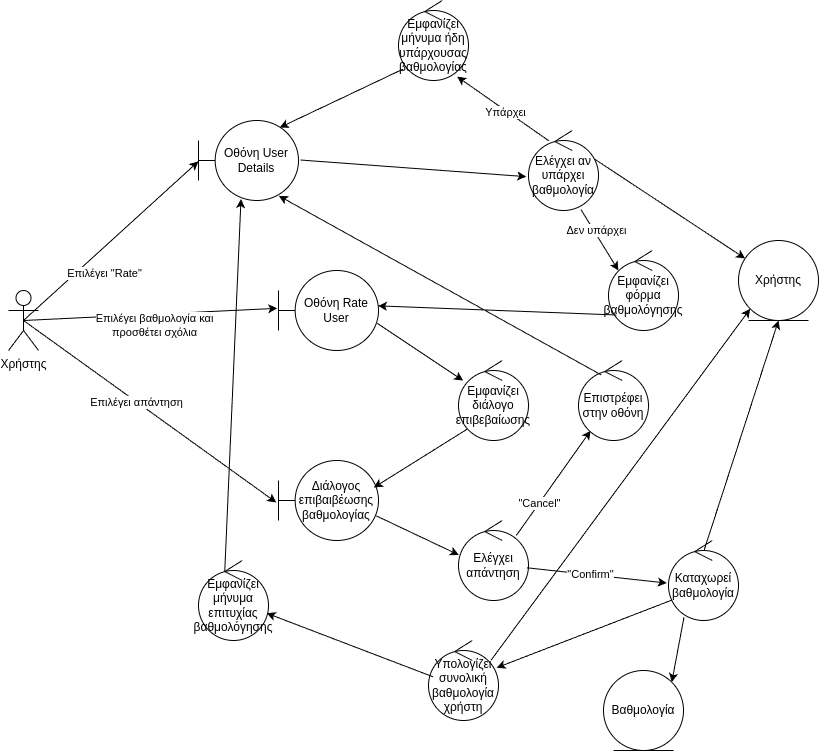
\includegraphics{./rate-user-robustness.drawio.png}
\caption{image}
\end{figure}

\subsection{Redeem Reward}

Ο χρήστης επιθυμεί να λάβει μια ανταμοιβή που έχει κερδίσει μέσω
της εφαρμογής.

\subsubsection{Βασική Ροή}

\begin{enumerate}
    \item Ο χρήστης επιλέγει "Redeem Reward"
    \item Η εφαρμογή υπολογίζει τους πόντους του χρήστη.
    \item Η εφαρμογή εμφανίζει τις διαθέσιμες ανταμοιβές και τους πόντους.
    \item Ο χρήστης επιλέγει την ανταμοιβή που επιθυμεί.
    \item Η εφαρμογή ενημερώνει τους πόντους του χρήστη και αφαιρεί την ανταμοιβή
          από τη λίστα των διαθέσιμων ανταμοιβών.
    \item Η εφαρμογή εμφανίζει τον κωδικό εξαργύρωσης.
\end{enumerate}

\subsubsection{Εναλλακτική Ροή: Ακύρωση}

\begin{enumerate}
    \item[4] Ο χρήστης εγκαταλείπει την διαδικασία.
\end{enumerate}

\subsubsection{Εναλλακτική Ροή: Δεν υπάρχουν διαθέσιμες ανταμοιβές}

\begin{enumerate}
    \item[3] Η εφαρμογή εμφανίζει μήνυμα ότι δεν υπάρχουν διαθέσιμες ανταμοιβές.
\end{enumerate}

\subsubsection{Εναλλακτική Ροή: Ανεπαρκής αριθμός πόντων}

\begin{enumerate}
    \item[5] Η εφαρμογή εμφανίζει μήνυμα ότι ο χρήστης δεν έχει αρκετούς πόντους.
    \item[6] Συνέχεια από το βήμα 3 της βασικής ροής.
\end{enumerate}

\subsection{Report User}

Ο χρήστης επιθυμεί να αναφέρει έναν άλλο χρήστη της εφαρμογής για
παράνομη ή ανεπιθύμητη δραστηριότητα.

\subsubsection{Βασική Ροή}

\begin{enumerate}
    \item Ο χρήστης επιλέγει τον χρήστη που θέλει να αναφέρει και πατάει "Report".
    \item H εφαρμογή εμφανίζει την φόρμα αναφοράς.
    \item Ο χρήστης επιλέγει τον λόγο αναφοράς, προσθέτει σχόλια και πατάει υποβολή.
    \item Η εφαρμογή ενημερώνει τον χρήστη για την επιτυχή υποβολή.
    \item Το σύστημα επεξεργάζεται την αναφορά και την τοποθετεί σε λίστα αναμονής.
\end{enumerate}

\subsubsection{Εναλλακτική Ροή: Ακύρωση}

\begin{enumerate}
    \item[3] Ο χρήστης αποφασίζει να μην υποβάλει την αναφορά και πατάει "Cancel".
\end{enumerate}

\hypertarget{view-past-rides}{%
\subsection{View Past Rides}\label{view-past-rides}}

\hypertarget{ux3c0ux3b5ux3c1ux3b9ux3b3ux3c1ux3b1ux3c6ux3ae}{%
\subsubsection{Περιγραφή}\label{ux3c0ux3b5ux3c1ux3b9ux3b3ux3c1ux3b1ux3c6ux3ae}}

Ο χρήστης επιθυμεί να δει το ιστορικό διαδρομών του.

\hypertarget{ux3b2ux3b1ux3c3ux3b9ux3baux3ae-ux3c1ux3bfux3ae}{%
\paragraph{Βασική
ροή}\label{ux3b2ux3b1ux3c3ux3b9ux3baux3ae-ux3c1ux3bfux3ae}}

\begin{enumerate}
\def\labelenumi{\arabic{enumi}.}
\tightlist
\item
  Ο χρήστης επιλέγει ``Past Rides'' στην οθόνη Account.
\item
  Το σύστημα ανακτά το ιστορικό διαδρομών και το εμφανίζει στην οθόνη
  Past Rides.
\item
  Ο χρήστης επιλέγει μία διαδρομή στην οθόνη Past Rides.
\item
  Το σύστημα εμφανίζει τις λεπτομέρειες της διαδρομής στην οθόνη Ride
  Details.
\end{enumerate}

\hypertarget{ux3b5ux3bdux3b1ux3bbux3bbux3b1ux3baux3c4ux3b9ux3baux3ae-ux3c1ux3bfux3ae-ux3b4ux3b9ux3b1ux3b3ux3c1ux3b1ux3c6ux3ae-ux3b4ux3b9ux3b1ux3b4ux3c1ux3bfux3bcux3aeux3c2-ux3b1ux3c0ux3cc-ux3c4ux3bf-ux3b9ux3c3ux3c4ux3bfux3c1ux3b9ux3baux3cc}{%
\paragraph{Εναλλακτική Ροή: Διαγραφή διαδρομής από το
ιστορικό}\label{ux3b5ux3bdux3b1ux3bbux3bbux3b1ux3baux3c4ux3b9ux3baux3ae-ux3c1ux3bfux3ae-ux3b4ux3b9ux3b1ux3b3ux3c1ux3b1ux3c6ux3ae-ux3b4ux3b9ux3b1ux3b4ux3c1ux3bfux3bcux3aeux3c2-ux3b1ux3c0ux3cc-ux3c4ux3bf-ux3b9ux3c3ux3c4ux3bfux3c1ux3b9ux3baux3cc}}

\begin{enumerate}
\def\labelenumi{\arabic{enumi}.}
\setcounter{enumi}{4}
\tightlist
\item
  Ο χρήστης επιλέγει ``Delete'' στην οθόνη Ride History.
\item
  Το σύστημα εμφανίζει τoν διάλογο επιβεβαίωσης διαγραφής.
\item
  Ο χρήστης επιλέγει ``Confirm'' στον διάλογο επιβεβαίωσης διαγραφής.
\item
  Το σύστημα διαγράφει τη διαδρομή από το ιστορικό.
\item
  Το σύστημα εμφανίζει μήνυμα επιτυχίας στην οθόνη Past Rides.
\end{enumerate}

\hypertarget{ux3b5ux3bdux3b1ux3bbux3bbux3b1ux3baux3c4ux3b9ux3baux3ae-ux3c1ux3bfux3ae-ux3b1ux3baux3cdux3c1ux3c9ux3c3ux3b7-ux3b4ux3b9ux3b1ux3b3ux3c1ux3b1ux3c6ux3aeux3c2}{%
\paragraph{Εναλλακτική Ροή: Ακύρωση
Διαγραφής}\label{ux3b5ux3bdux3b1ux3bbux3bbux3b1ux3baux3c4ux3b9ux3baux3ae-ux3c1ux3bfux3ae-ux3b1ux3baux3cdux3c1ux3c9ux3c3ux3b7-ux3b4ux3b9ux3b1ux3b3ux3c1ux3b1ux3c6ux3aeux3c2}}

\begin{enumerate}
\def\labelenumi{\arabic{enumi}.}
\setcounter{enumi}{4}
\tightlist
\item
  Ο χρήστης επιλέγει ``Delete'' στην οθόνη Ride History.
\item
  Το σύστημα εμφανίζει τoν διάλογο επιβεβαίωσης διαγραφής.
\item
  Ο χρήστης επιλέγει ``Cancel'' στον διάλογο επιβεβαίωσης διαγραφής.
\item
  Το σύστημα επιστρέφει στην οθόνη Past Rides.
\end{enumerate}

\hypertarget{ux3b1ux3bdux3acux3bbux3c5ux3c3ux3b7-ux3b5ux3c5ux3c1ux3c9ux3c3ux3c4ux3afux3b1ux3c2}{%
\subsubsection{Ανάλυση
Ευρωστίας}\label{ux3b1ux3bdux3acux3bbux3c5ux3c3ux3b7-ux3b5ux3c5ux3c1ux3c9ux3c3ux3c4ux3afux3b1ux3c2}}

\begin{figure}
\centering
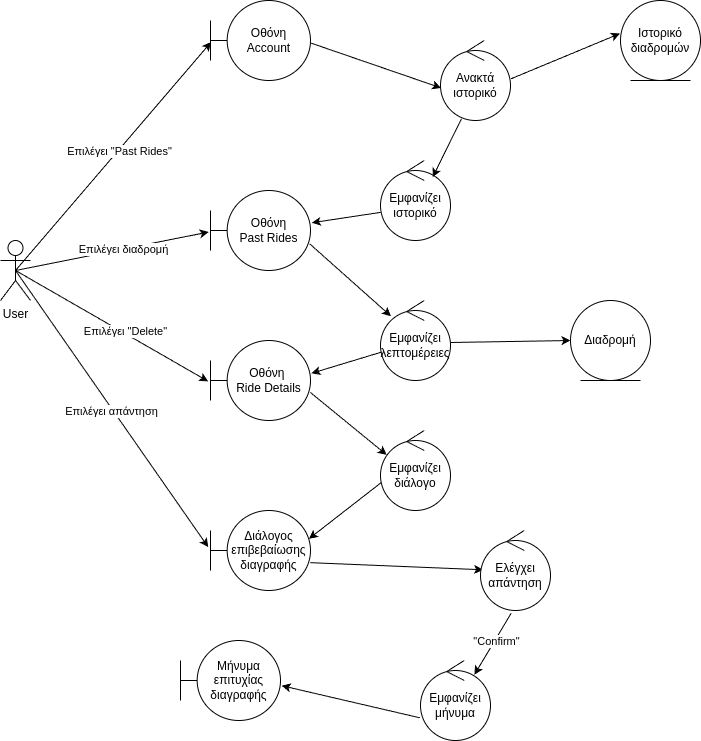
\includegraphics{./view-past-rides-robustness.drawio.png}
\caption{image}
\end{figure}

\section{Robustness Diagrams}
\subsection{Arrange Pickup}
\includegraphics[width=\textwidth]{build/robustness/arrange-pickup.png}
\subsection{Confirm Pickup}
\includegraphics[width=\textwidth]{build/robustness/confirm-pickup.png}
\subsection{Create Activity}
\includegraphics[width=\textwidth]{build/robustness/create-activity.png}
\subsection{Create ride}
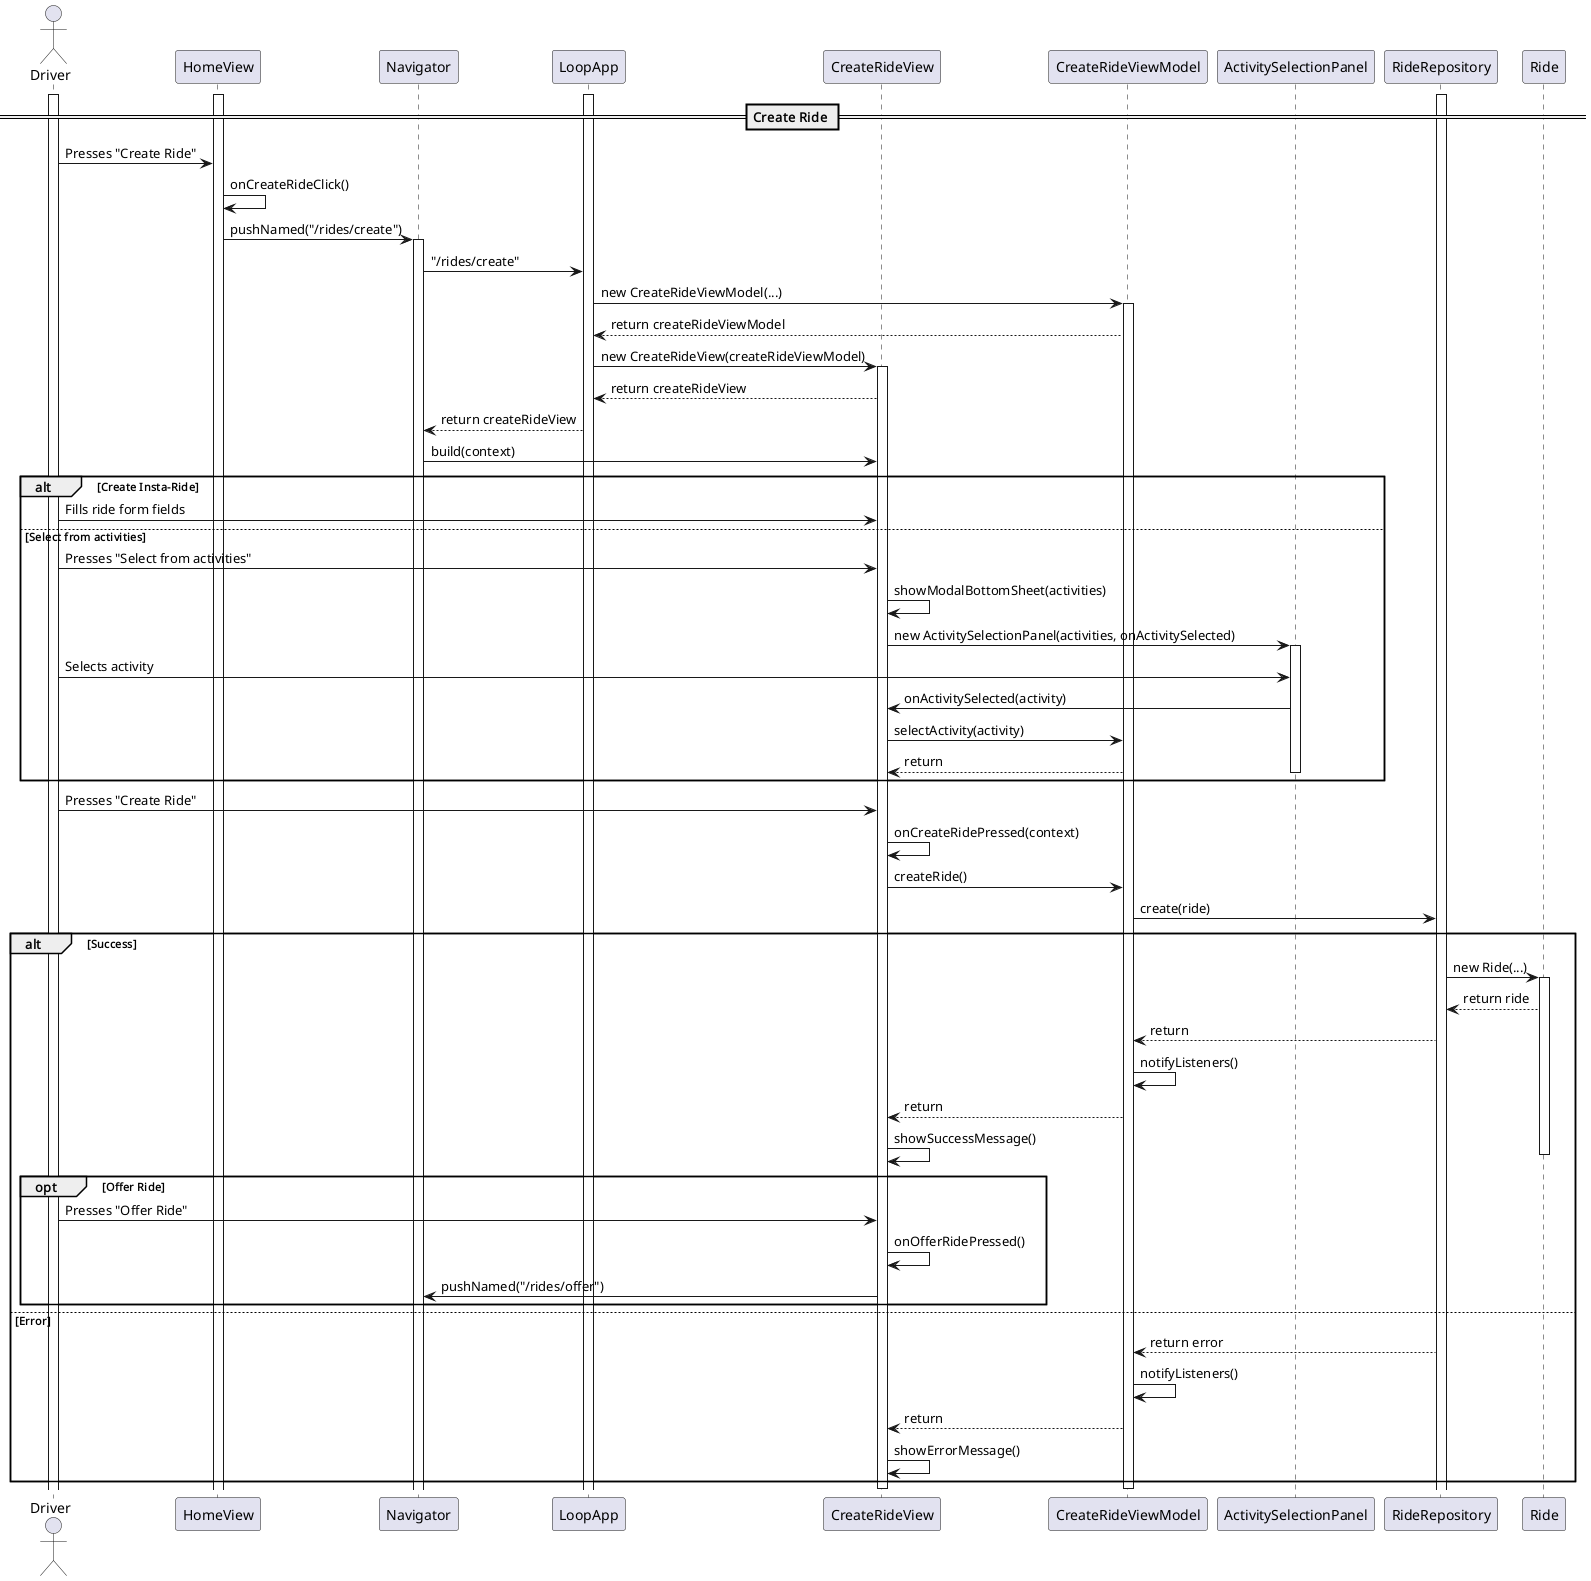
\includegraphics[width=\textwidth]{build/robustness/create-ride.png}
\subsection{Edit Activity}
\includegraphics[width=\textwidth]{build/robustness/edit-activity.png}
\subsection{Edit Profile}
\includegraphics[width=\textwidth]{build/robustness/edit-profile.png}
\subsection{Find Ride}
\includegraphics[width=\textwidth]{build/robustness/find-ride.png}
\subsection{Join Ride}
\includegraphics[width=\textwidth]{build/robustness/join-ride.png}
\subsection{Manage ride}
No diagram found for manage-ride
\subsection{Offer Ride}
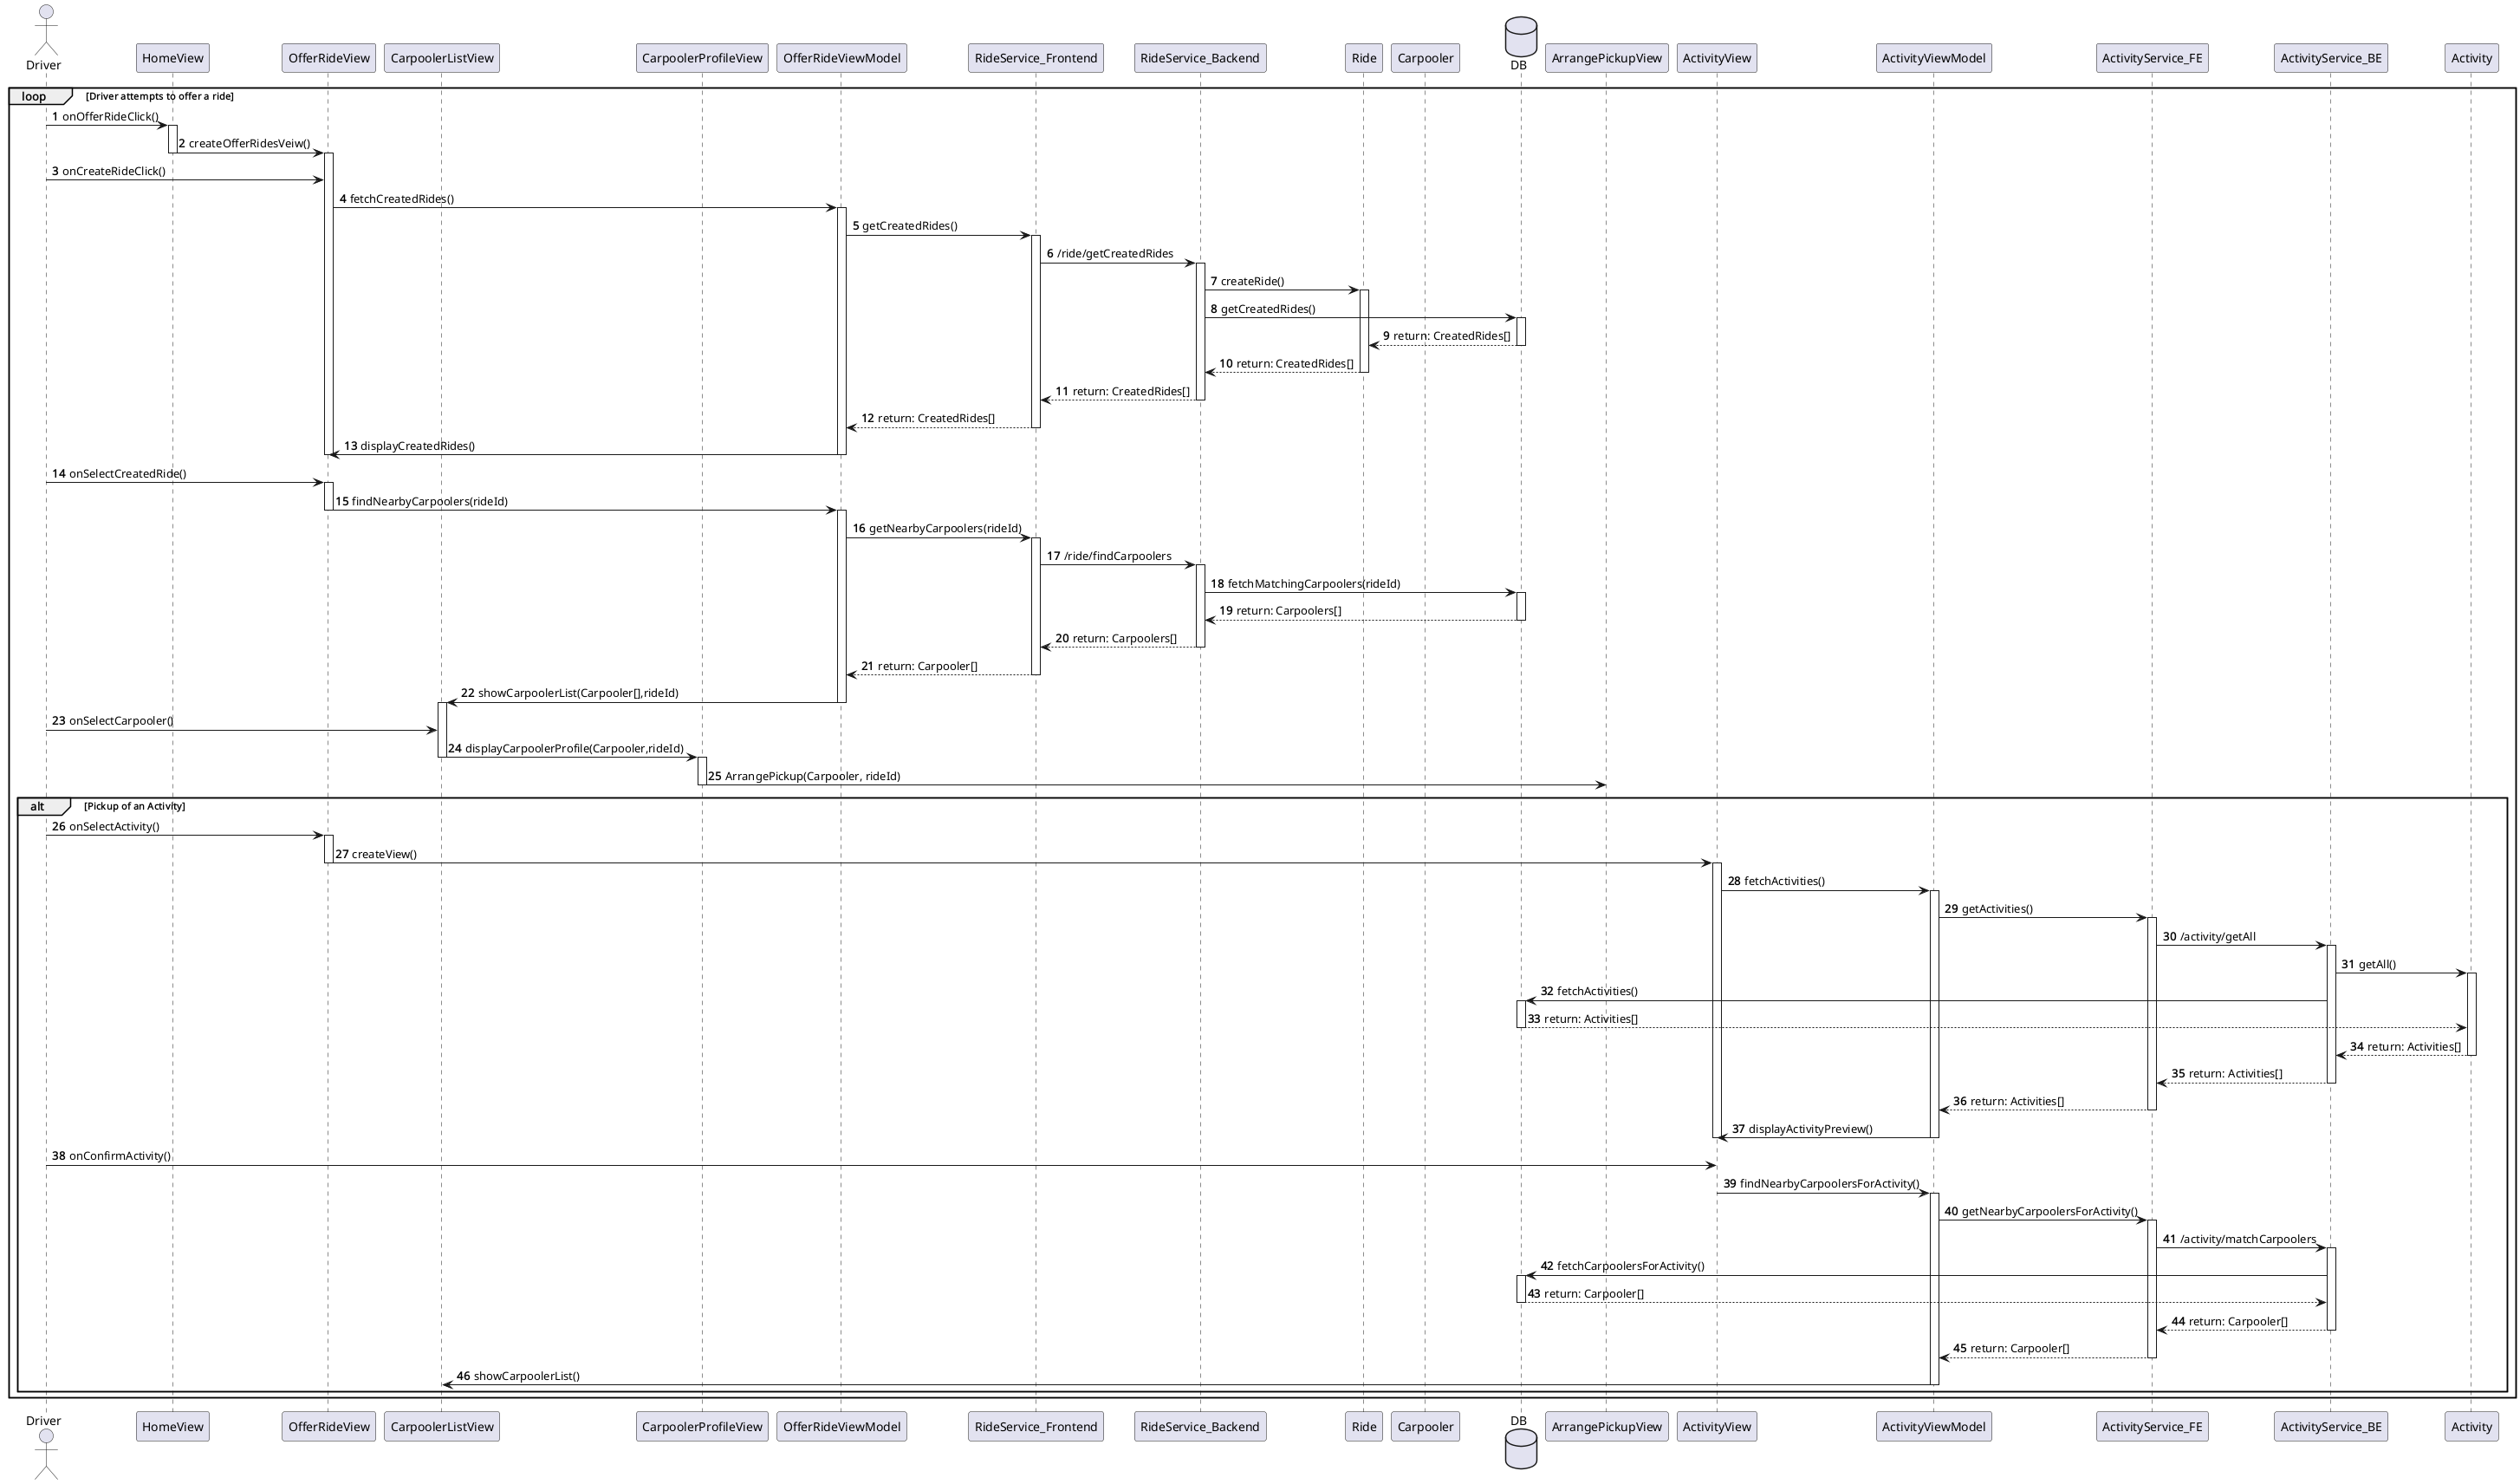
\includegraphics[width=\textwidth]{build/robustness/offer-ride.png}
\subsection{Rate User}
\includegraphics[width=\textwidth]{build/robustness/rate-user.png}
\subsection{Redeem Reward}
\includegraphics[width=\textwidth]{build/robustness/redeem-reward.png}
\subsection{Report User}
\includegraphics[width=\textwidth]{build/robustness/report-user.png}
\subsection{View Past Rides}
\includegraphics[width=\textwidth]{build/robustness/view-past-rides.png}
\section{Sequence Diagrams}
\subsection{Arrange Pickup}
\includegraphics[width=\textwidth]{build/sequence/arrange-pickup.png}
\subsection{Confirm Pickup}
No diagram found for confirm-pickup
\subsection{Create Activity}
No diagram found for create-activity
\subsection{Create ride}
No diagram found for create-ride
\subsection{Edit Activity}
No diagram found for edit-activity
\subsection{Edit Profile}
\includegraphics[width=\textwidth]{build/sequence/edit-profile.png}
\subsection{Find Ride}
\includegraphics[width=\textwidth]{build/sequence/find-ride.png}
\subsection{Join Ride}
\includegraphics[width=\textwidth]{build/sequence/join-ride.png}
\subsection{Manage ride}
No diagram found for manage-ride
\subsection{Offer Ride}
No diagram found for offer-ride
\subsection{Rate User}
\includegraphics[width=\textwidth]{build/sequence/rate-user.png}
\subsection{Redeem Reward}
\includegraphics[width=\textwidth]{build/sequence/redeem-reward.png}
\subsection{Report User}
\includegraphics[width=\textwidth]{build/sequence/report-user.png}
\subsection{View Past Rides}
\includegraphics[width=\textwidth]{build/sequence/view-past-rides.png}


% \newpage

% \section{Ενδεικτικές Οθόνες}

% \subsection{Κεντρική Οθόνη}

% \begin{figure}[H]
%     \centering
%     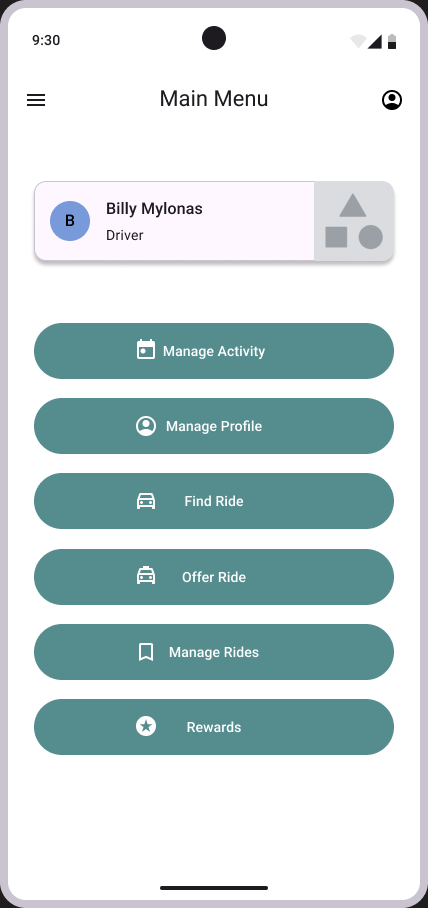
\includegraphics[width=0.9\textwidth]{reports/mockups/main-menu}
%     \caption{Κεντρική Οθόνη}
% \end{figure}

% \subsection{Εύρεση Διαδρομής (Find Ride)}

% \begin{figure}[H]
%     \centering
%     \begin{subfigure}[b]{0.28\textwidth}
%         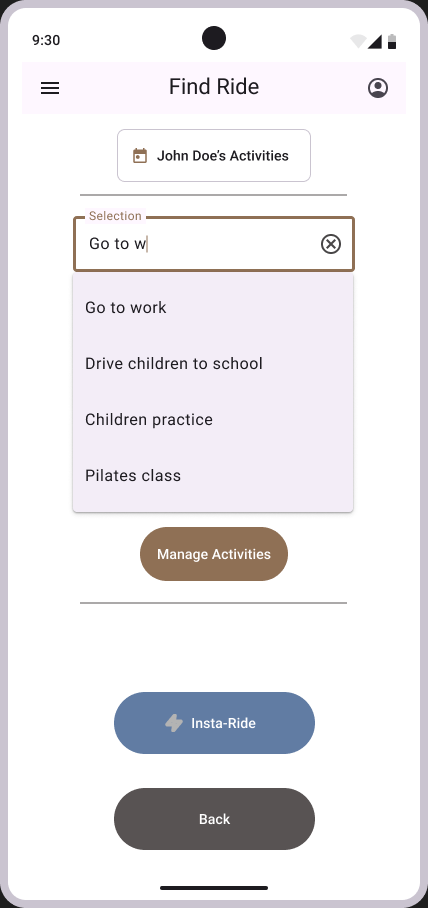
\includegraphics[width=\textwidth]{reports/mockups/find-ride-1}
%         \caption{Επιλογή διαδρομής μέσω Activity}
%     \end{subfigure}
%     \hfill
%     \begin{subfigure}[b]{0.28\textwidth}
%         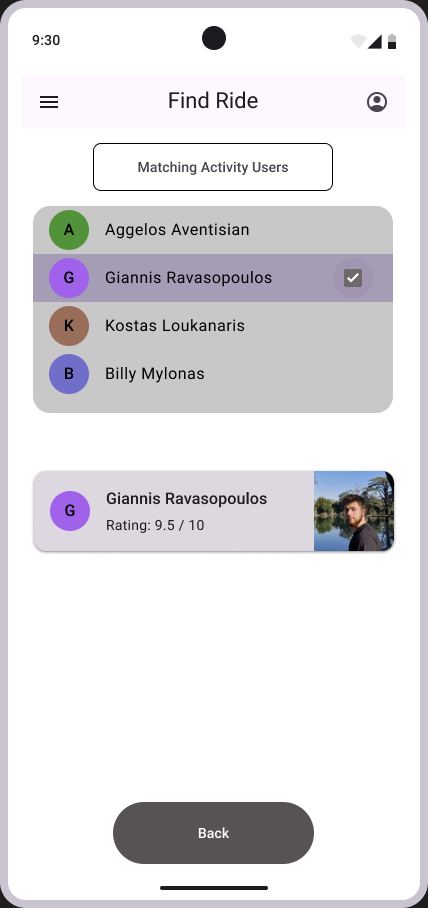
\includegraphics[width=\textwidth]{reports/mockups/find-ride-2}
%         \caption{Επιλογή συνεπιβατών}
%     \end{subfigure}
%     \hfill
%     \begin{subfigure}[b]{0.28\textwidth}
%         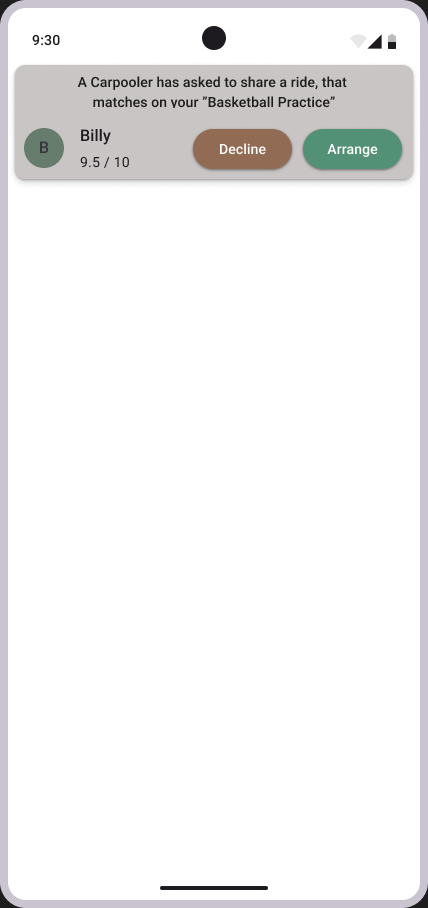
\includegraphics[width=\textwidth]{reports/mockups/find-ride-3}
%         \caption{Ειδοποίηση οδηγού}
%     \end{subfigure}
%     \caption{Διαδικασία εύρεσης διαδρομής}
% \end{figure}

% \begin{figure}[H]
%     \centering
%     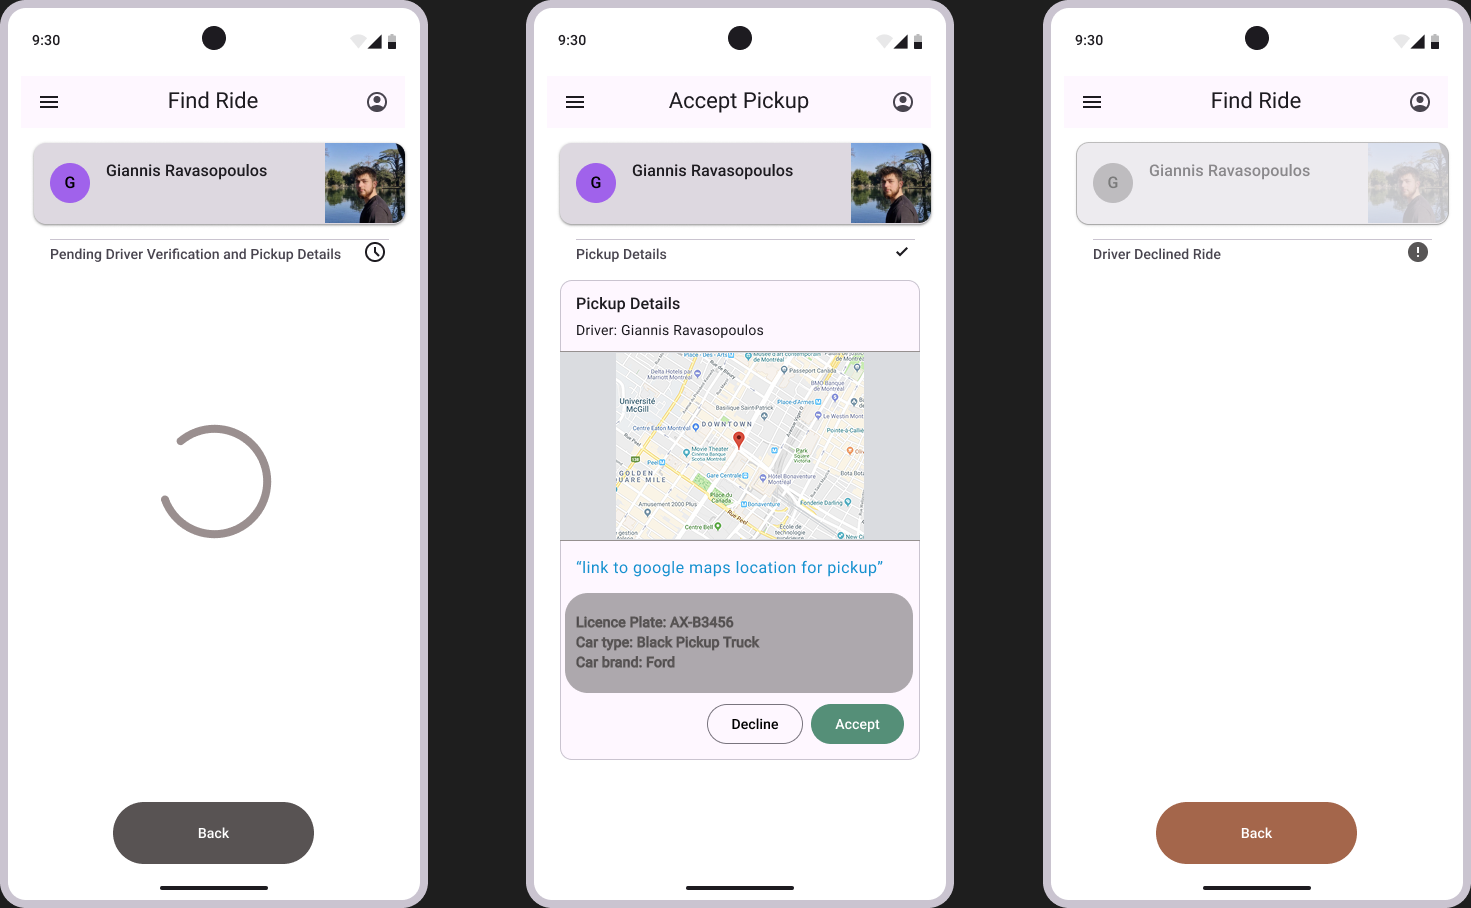
\includegraphics[width=0.9\textwidth]{reports/mockups/find-ride-4}
%     \caption{Επιβεβαίωση σημείου παραλαβής (2: σενάριο αποδοχής από τον οδηγό, 3: σενάριο απόρριψης από τον οδηγό)}
% \end{figure}

% \newpage

% \begin{figure}[H]
%     \centering
%     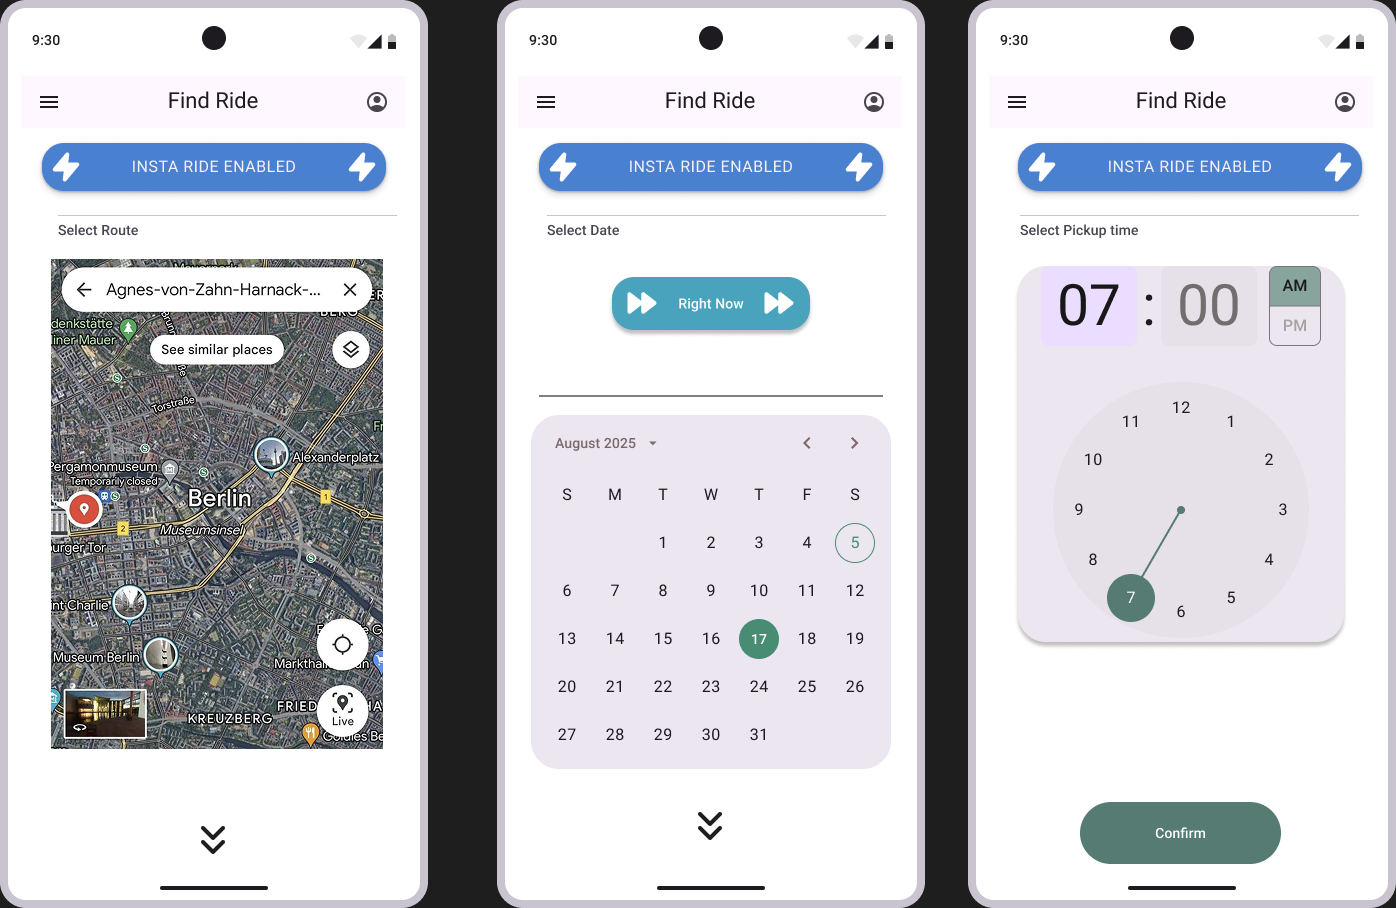
\includegraphics[width=\textwidth]{reports/mockups/find-ride-1b}
%     \caption{Επιλογή διαδρομής μέσω Insta-Ride}
% \end{figure}

% \newpage

% \subsection{Προσφορά Διαδρομής (Offer Ride)}

% \begin{figure}[H]
%     \centering
%     \begin{subfigure}[b]{0.3\textwidth}
%         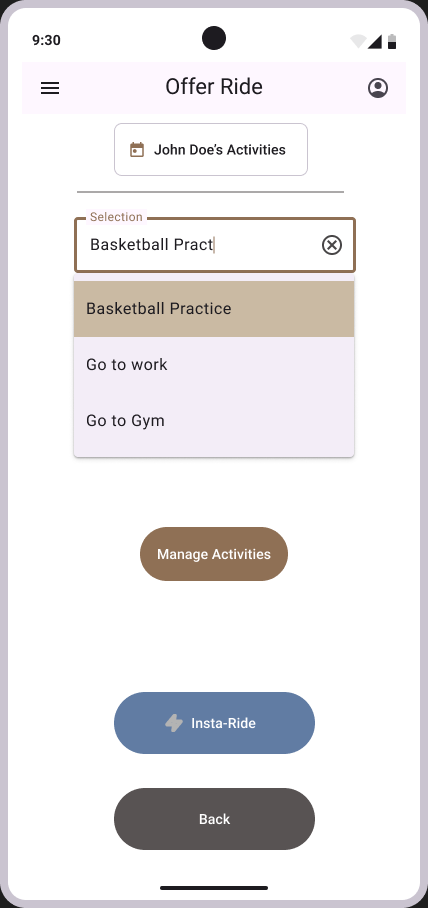
\includegraphics[width=\textwidth]{reports/mockups/offer-ride-1}
%         \caption{Επιλογή διαδρομής μέσω Activity}
%     \end{subfigure}
%     \hfill
%     \begin{subfigure}[b]{0.3\textwidth}
%         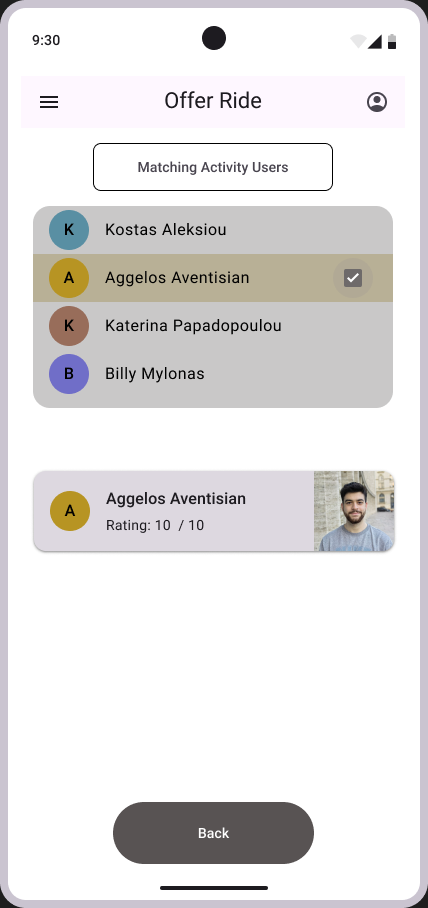
\includegraphics[width=\textwidth]{reports/mockups/offer-ride-2}
%         \caption{Επιλογή οδηγού}
%     \end{subfigure}
% \end{figure}

% \begin{figure}[H]
%     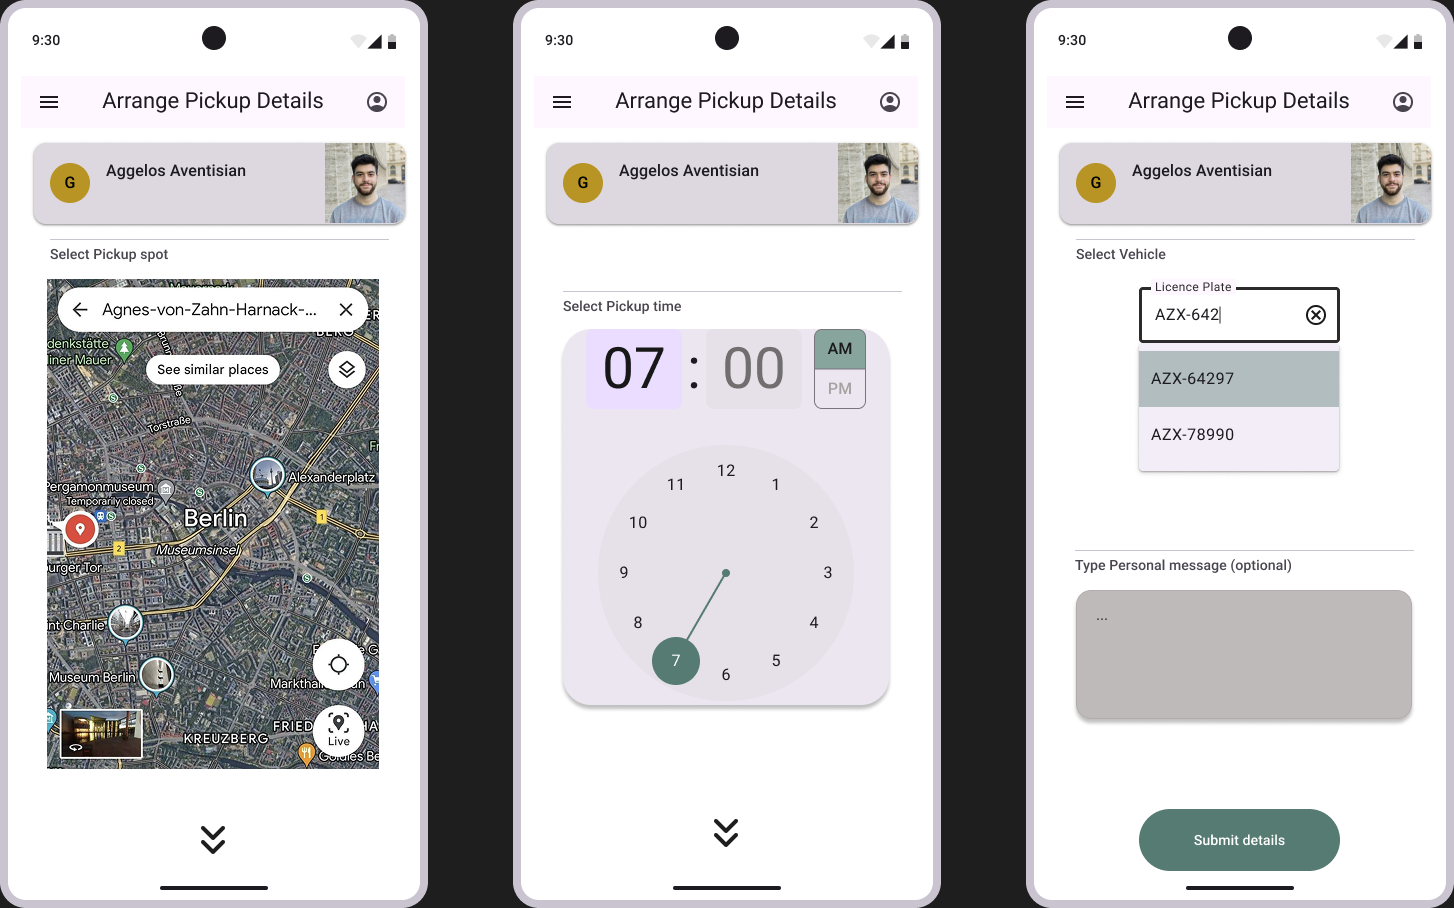
\includegraphics[width=0.9\textwidth]{reports/mockups/offer-ride-3a}
%     \caption{Επιλογή σημείου και ώρας παραλαβής}
% \end{figure}

% \newpage

% \begin{figure}[h!]
%     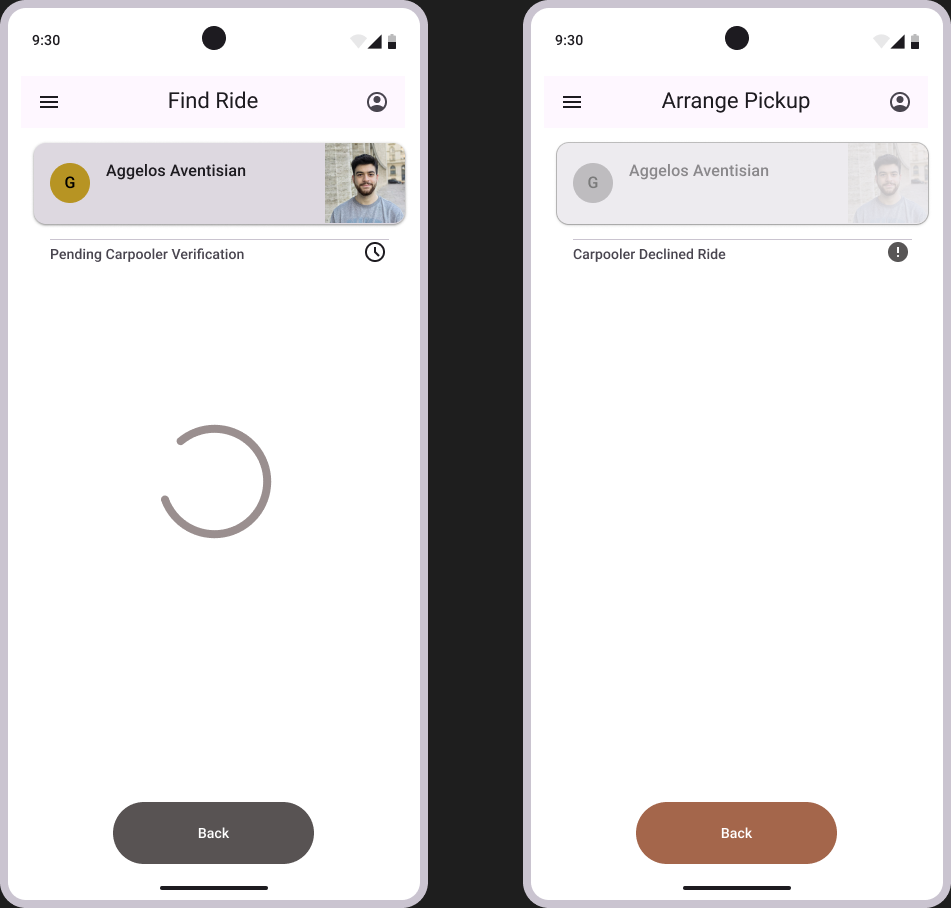
\includegraphics[width=\textwidth]{reports/mockups/offer-ride-3b}
%     \caption{Απόρριψη από τον Carpooler}
% \end{figure}

% \newpage

% \subsection{Manage Ride}

% \begin{figure}[H]
%     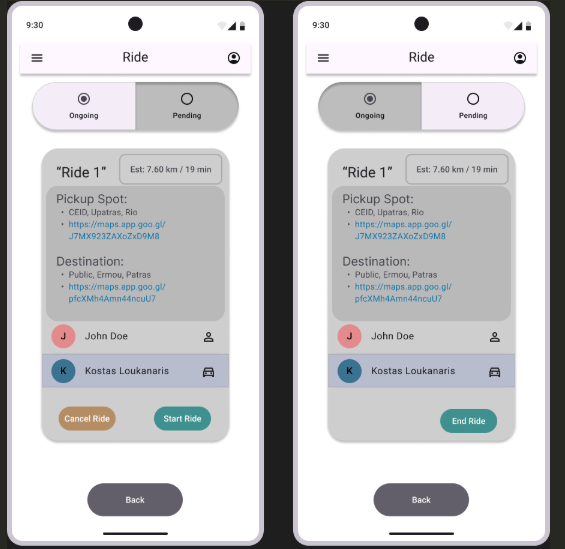
\includegraphics[width=\textwidth]{reports/mockups/image}
%     \caption{Έναρξη διαδρομής (Start Ride)}
% \end{figure}

% \newpage

% \subsection{Εξαργύρωση ανταμοιβής (Redeem Reward)}

% \begin{figure}[H]
%     \centering
%     \begin{subfigure}[b]{0.3\textwidth}
%         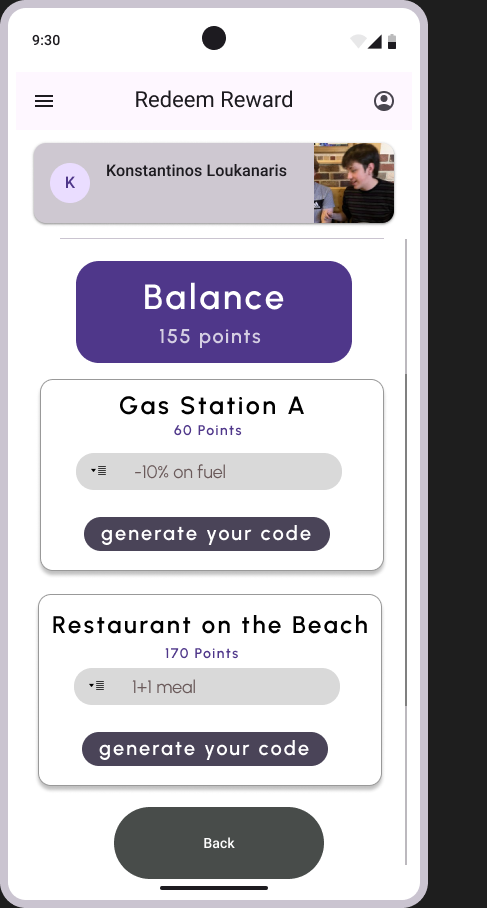
\includegraphics[width=\textwidth]{reports/mockups/redeem-reward-3}
%         \caption{Εμφάνιση Κουπονιών και πόντων}
%     \end{subfigure}
%     \hfill
%     \begin{subfigure}[b]{0.3\textwidth}
%         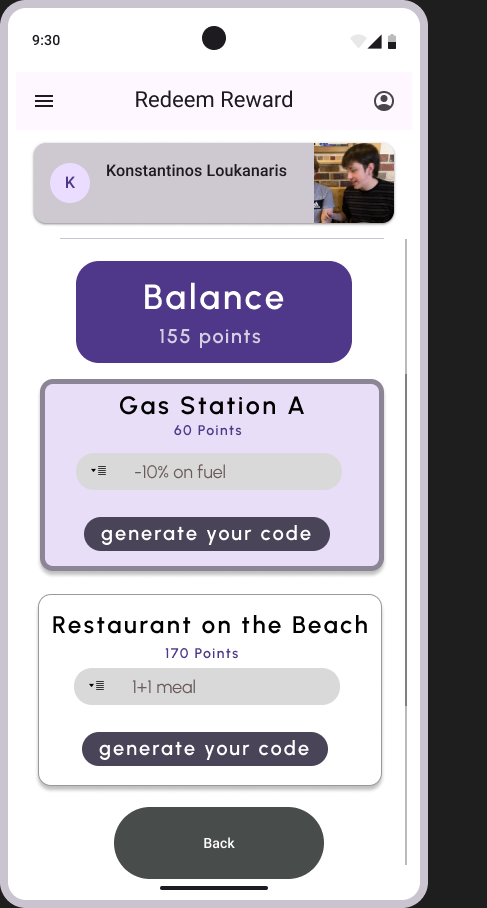
\includegraphics[width=\textwidth]{reports/mockups/redeem-reward-4}
%         \caption{Επιλογή κουπονιού}
%     \end{subfigure}
%     \hfill
%     \begin{subfigure}[b]{0.3\textwidth}
%         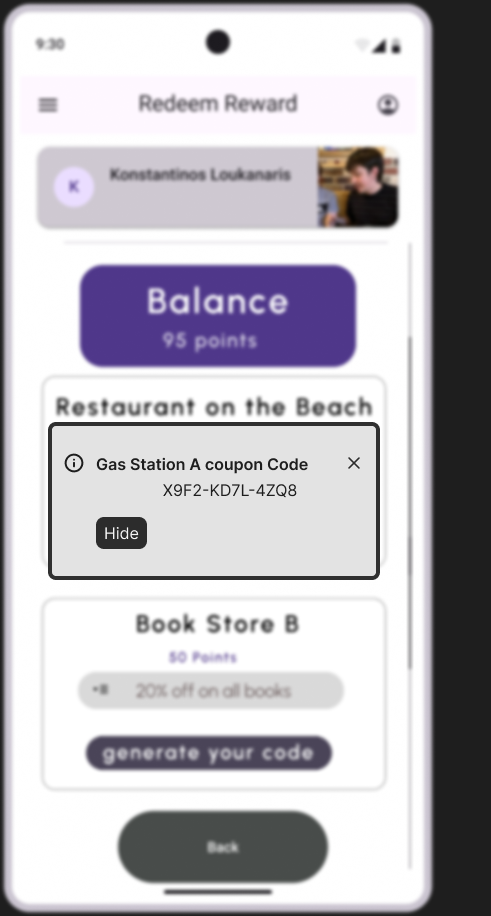
\includegraphics[width=0.9\textwidth]{reports/mockups/redeem-reward-5}
%         \caption{Επιβεβαίωση εξαργύρωσης και εμφάνιση κωδικού κουπονιού}
%     \end{subfigure}
% \end{figure}

% \newpage

% \subsection{Λοιπές Οθόνες}

% \begin{figure}[H]
%     \centering
%     \begin{subfigure}[b]{0.3\textwidth}
%         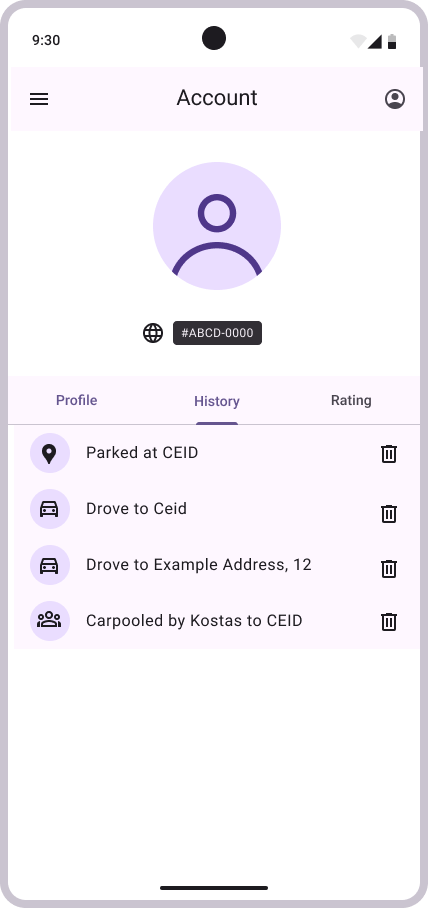
\includegraphics[width=\textwidth]{reports/mockups/history}
%         \caption{Προβολή Ιστορικού}
%     \end{subfigure}
%     \hfill
%     \begin{subfigure}[b]{0.3\textwidth}
%         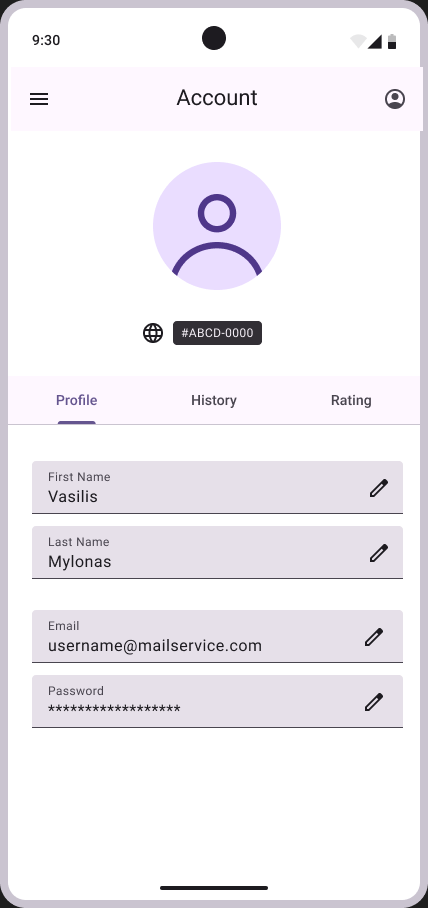
\includegraphics[width=\textwidth]{reports/mockups/profile}
%         \caption{Προβολή Προφίλ}
%     \end{subfigure}
%     \hfill
%     \begin{subfigure}[b]{0.3\textwidth}
%         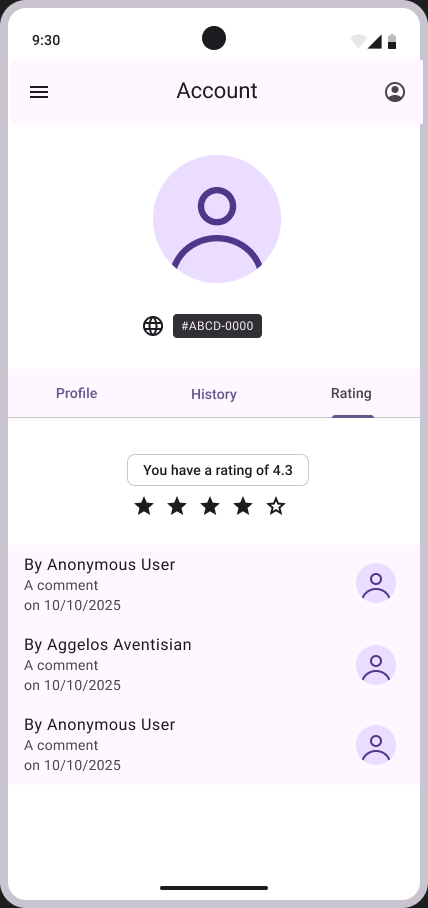
\includegraphics[width=\textwidth]{reports/mockups/rating}
%         \caption{Προβολή Βαθμολογίας}
%     \end{subfigure}
%     \caption{}
% \end{figure}

\end{document}
